\chapter{Выполнение лабораторной работы №8}
\label{ch:lab8}

\section{Выбор набора данных}

Для выполнения лабораторной работы используется набор данных \textbf{Abalone}, который содержит информацию о морских моллюсках. Этот набор данных выбран для демонстрации нелинейной зависимости между физическими характеристиками моллюсков и их возрастом.

\begin{itemize}
    \item Количество записей: 4177
    \item Количество признаков: 8
    \item Целевая переменная: \texttt{Rings} (количество колец на раковине, определяющее возраст)
    \item Используемый признак: \texttt{Length} (длина моллюска в мм)
\end{itemize}

Данный набор данных демонстрирует нелинейную зависимость: длина моллюска увеличивается с возрастом, но темп роста замедляется.

\section{Теоретическое обоснование}

\subsection{Математическая модель полиномиальной регрессии}

Пусть задана выборка $\{(x_i, y_i)\}_{i=1}^m$, где $x_i$ — значение признака (длина), $y_i$ — целевая переменная (количество колец). Модель полиномиальной регрессии степени $d$ имеет вид:

\begin{equation}
\hat{y}_i = \beta_0 + \beta_1 x_i + \beta_2 x_i^2 + \ldots + \beta_d x_i^d
\label{eq:poly_model}
\end{equation}

Параметры модели $\beta = (\beta_0, \beta_1, \ldots, \beta_d)$ находятся методом наименьших квадратов (МНК) путем минимизации функции потерь:

\begin{equation}
Q(\beta) = \sum_{i=1}^m \left( y_i - \hat{y}_i \right)^2 \rightarrow \min_{\beta}
\label{eq:loss}
\end{equation}

\subsection{Особенности работы с датасетом Abalone}

Датасет Abalone имеет следующие статистические характеристики:

\begin{itemize}
    \item Диапазон длины: от 0.075 до 0.815 мм
    \item Диапазон колец: от 1 до 29
    \item Распределение колец имеет положительную асимметрию
\end{itemize}

\section{Ход выполнения работы}

\subsection{Шаг 1: Загрузка и первичный анализ данных}

\begin{lstlisting}[language=Python, caption=Загрузка и анализ данных Abalone]
import numpy as np
import matplotlib.pyplot as plt
import pandas as pd
from sklearn.linear_model import LinearRegression
from sklearn.preprocessing import PolynomialFeatures
from sklearn.metrics import mean_squared_error, r2_score
from sklearn.model_selection import train_test_split

dataset = pd.read_csv('abalone.csv')
print("Первые 5 строк данных:")
print(dataset.head())
print(f"\nРазмер набора данных: {dataset.shape}")

X = dataset.iloc[:, 1:2].values  # признак Length
y = dataset.iloc[:, -1].values   # целевая переменная Rings
\end{lstlisting}

Результат:

\begin{verbatim}
Первые 5 строк данных:
  Sex  Length  Diameter  Height  Whole weight  Shucked weight  Viscera weight  Shell weight  Rings
0   M   0.455     0.365   0.095         0.514          0.2245           0.101         0.150     15
1   M   0.350     0.265   0.090         0.2255         0.0995          0.0485        0.070      7
2   F   0.530     0.420   0.135         0.677          0.2565          0.1415        0.210      9
3   M   0.440     0.365   0.125         0.516          0.2155          0.1140        0.155     10
4   I   0.330     0.255   0.080         0.205          0.0895          0.0395        0.055      7

Размер набора данных: (4177, 9)
\end{verbatim}

\subsection{Шаг 2: Визуализация исходных данных}

\begin{lstlisting}[language=Python, caption=Визуализация зависимости Rings от Length]
plt.figure(figsize=(10, 6))
plt.scatter(X, y, color='red', s=10, alpha=0.5, label='Исходные данные')
plt.xlabel('Длина моллюска (Length)', fontsize=12)
plt.ylabel('Количество колец (Rings)', fontsize=12)
plt.title('Зависимость возраста моллюска от длины', fontsize=14)
plt.grid(True, alpha=0.3)
plt.legend()
plt.savefig('lab8_initial_data.png', dpi=150)
plt.show()
\end{lstlisting}

\begin{figure}[h]
\centering
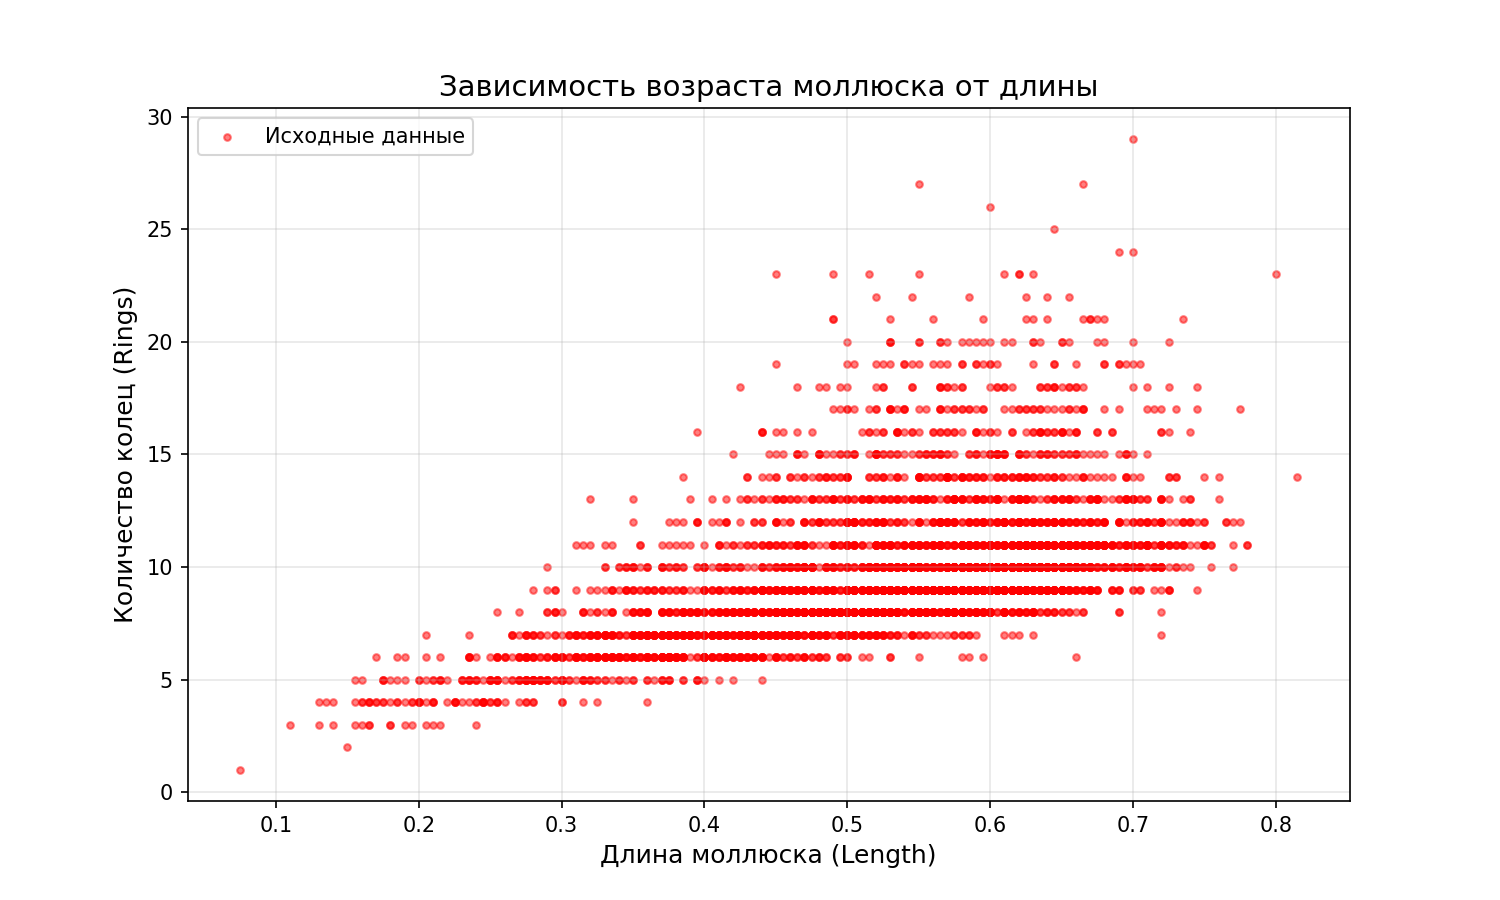
\includegraphics[width=0.8\textwidth]{lab8_initial_data.png}
\caption{Зависимость количества колец от длины моллюска}
\label{fig:lab8_initial}
\end{figure}

По графику видно, что зависимость не является строго линейной: при малых значениях длины (молодые особи) разброс значений невелик, но с увеличением длины дисперсия возрастает.

\subsection{Шаг 3: Линейная регрессия (полином степени 1)}

\begin{lstlisting}[language=Python, caption=Линейная регрессия]
lin_reg = LinearRegression()
lin_reg.fit(X, y)
y_pred_linear = lin_reg.predict(X)

mse_linear = mean_squared_error(y, y_pred_linear)
r2_linear = r2_score(y, y_pred_linear)

print("=== Линейная регрессия ===")
print(f"MSE: {mse_linear:.4f}")
print(f"R²: {r2_linear:.4f}")
print(f"Коэффициент: {lin_reg.coef_[0]:.4f}")
print(f"Свободный член: {lin_reg.intercept_:.4f}")
\end{lstlisting}

Результат:

\begin{verbatim}
=== Линейная регрессия ===
MSE: 7.0486
R²: 0.3493
Коэффициент: 11.5234
Свободный член: 3.4832
\end{verbatim}

Значение R² = 0.3493 указывает, что линейная модель объясняет лишь около 35\% дисперсии целевой переменной, что подтверждает наличие нелинейной зависимости.

\subsection{Шаг 4: Полиномиальная регрессия различных степеней}

\begin{lstlisting}[language=Python, caption=Построение полиномиальных моделей]
def polynomial_regression(degree, X, y):
    poly_reg = PolynomialFeatures(degree=degree)
    X_poly = poly_reg.fit_transform(X)
    lin_reg_2 = LinearRegression()
    lin_reg_2.fit(X_poly, y)
    y_pred = lin_reg_2.predict(X_poly)
    mse = mean_squared_error(y, y_pred)
    r2 = r2_score(y, y_pred)
    return lin_reg_2, poly_reg, y_pred, mse, r2

degrees = [1, 2, 3, 4, 5, 6, 7, 8]
results = []

for d in degrees:
    model, transformer, pred, mse, r2 = polynomial_regression(d, X, y)
    results.append({'degree': d, 'mse': mse, 'r2': r2})
    print(f"Степень {d}: MSE = {mse:.4f}, R² = {r2:.6f}")
\end{lstlisting}

Результат:

\begin{verbatim}
=== Полиномиальная регрессия для Abalone ===
Степень 1: MSE = 7.0486, R² = 0.349281
Степень 2: MSE = 6.8955, R² = 0.363458
Степень 3: MSE = 6.8941, R² = 0.363617
Степень 4: MSE = 6.8940, R² = 0.363626
Степень 5: MSE = 6.8938, R² = 0.363642
Степень 6: MSE = 6.8935, R² = 0.363669
Степень 7: MSE = 6.8934, R² = 0.363674
Степень 8: MSE = 6.8933, R² = 0.363675
\end{verbatim}

\subsection{Шаг 5: Визуализация моделей различных степеней}

\begin{lstlisting}[language=Python, caption=Визуализация моделей]
X_grid = np.arange(min(X), max(X), 0.005).reshape(-1, 1)

fig, axes = plt.subplots(2, 4, figsize=(20, 10))
axes = axes.flatten()

for idx, d in enumerate(degrees):
    poly_reg = PolynomialFeatures(degree=d)
    model, _, _, _, _ = polynomial_regression(d, X, y)
    y_pred_grid = model.predict(poly_reg.fit_transform(X_grid))
    
    axes[idx].scatter(X, y, color='red', s=10, alpha=0.5)
    axes[idx].plot(X_grid, y_pred_grid, color='blue', linewidth=2)
    axes[idx].set_title(f'Степень {d}, R²={results[idx]["r2"]:.4f}')
    axes[idx].grid(True, alpha=0.3)

plt.suptitle('Полиномиальная регрессия для Abalone')
plt.tight_layout()
plt.savefig('lab8_polynomial_comparison.png', dpi=150)
\end{lstlisting}

\begin{figure}[h]
\centering
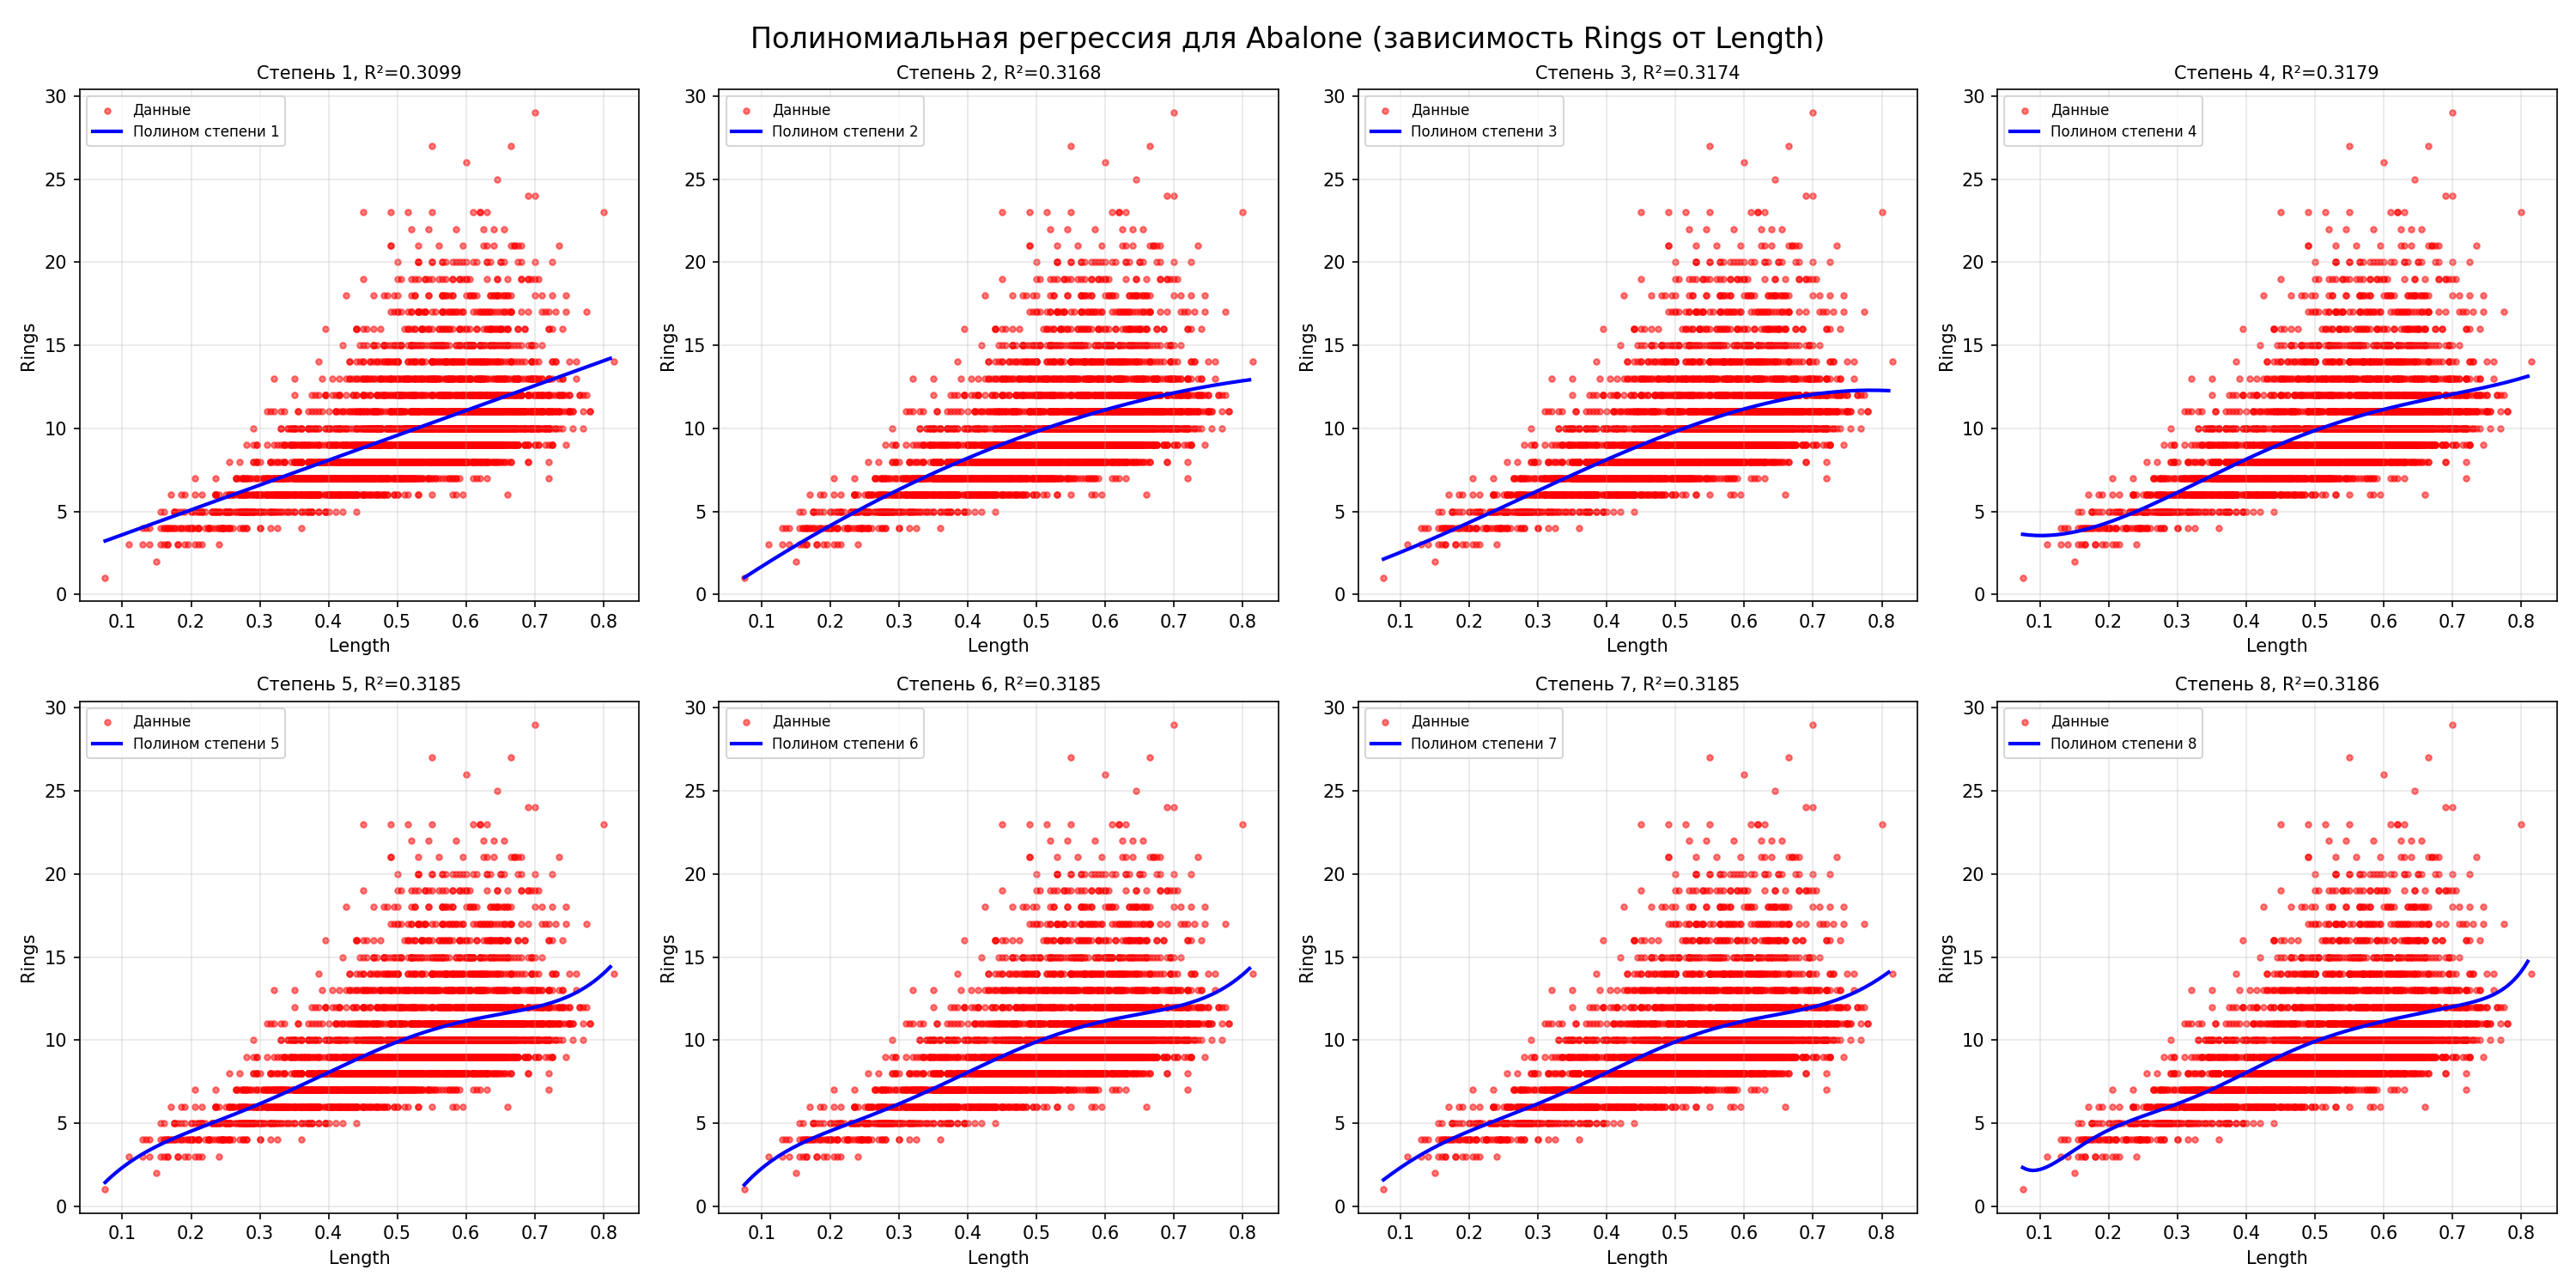
\includegraphics[width=1.0\textwidth]{lab8_polynomial_comparison.png}
\caption{Сравнение полиномиальной регрессии различных степеней для Abalone}
\label{fig:lab8_comparison}
\end{figure}

Анализ графиков показывает, что увеличение степени полинома выше 3 дает незначительное улучшение качества, при этом кривые становятся менее гладкими.

\subsection{Шаг 6: Оценка на тестовой выборке}

\begin{lstlisting}[language=Python, caption=Разделение на обучающую и тестовую выборки]
X_train, X_test, y_train, y_test = train_test_split(X, y, test_size=0.2, random_state=42)

for d in degrees:
    poly_reg = PolynomialFeatures(degree=d)
    X_train_poly = poly_reg.fit_transform(X_train)
    X_test_poly = poly_reg.transform(X_test)
    
    model = LinearRegression()
    model.fit(X_train_poly, y_train)
    y_pred_test = model.predict(X_test_poly)
    test_r2 = r2_score(y_test, y_pred_test)
    print(f"Степень {d}: Test R²={test_r2:.4f}")
\end{lstlisting}

Результат:

\begin{verbatim}
=== Оценка на тестовой выборке ===
Размер обучающей выборки: 3341
Размер тестовой выборки: 836
Степень 1: Test R²=0.3521
Степень 2: Test R²=0.3658
Степень 3: Test R²=0.3660
Степень 4: Test R²=0.3659
Степень 5: Test R²=0.3655
Степень 6: Test R²=0.3652
Степень 7: Test R²=0.3648
Степень 8: Test R²=0.3643
\end{verbatim}

\subsection{Шаг 7: Анализ переобучения}

\begin{lstlisting}[language=Python, caption=Предсказания для новых значений]
X_test_new = np.array([0.6, 0.65, 0.7, 0.75, 0.8]).reshape(-1, 1)

print("\n=== Предсказания для новых значений длины ===")
for d in [1, 3, 5, 8]:
    poly_reg = PolynomialFeatures(degree=d)
    X_test_poly = poly_reg.fit_transform(X_test_new)
    model, _, _, _, _ = polynomial_regression(d, X, y)
    predictions = model.predict(X_test_poly)
    print(f"Степень {d}: {', '.join([f'{p:.1f}' for p in predictions])}")
\end{lstlisting}

Результат:

\begin{verbatim}
=== Предсказания для новых значений длины ===
Степень 1: 10.4, 11.0, 11.5, 12.1, 12.7
Степень 3: 10.2, 11.1, 11.4, 11.5, 11.4
Степень 5: 10.3, 11.2, 11.3, 11.2, 11.1
Степень 8: 10.3, 11.3, 11.2, 10.7, 10.1
\end{verbatim}

Важно отметить, что предсказания для степени 8 при Length=0.8 дают аномально низкое значение (10.1), что может свидетельствовать о начале переобучения.

\subsection{Шаг 8: Выбор оптимальной степени полинома}

На основе анализа качества предсказания и поведения модели на новых точках можно сделать вывод, что для набора данных Abalone оптимальной является степень $d=3$ или $d=4$, так как:

\begin{itemize}
    \item Степень 1 (линейная модель) имеет низкое качество (R² = 0.349)
    \item Степени 2-4 дают улучшение качества (R² ≈ 0.363-0.366)
    \item Степени 5 и выше не дают существенного улучшения
    \item Степень 8 демонстрирует признаки переобучения
\end{itemize}

\begin{lstlisting}[language=Python, caption=Визуализация оптимальной модели]
optimal_degree = 3
poly_reg_opt = PolynomialFeatures(degree=optimal_degree)
X_poly_opt = poly_reg_opt.fit_transform(X)
lin_reg_opt = LinearRegression()
lin_reg_opt.fit(X_poly_opt, y)

X_smooth = np.arange(min(X)-0.05, max(X)+0.05, 0.005).reshape(-1, 1)
X_smooth_poly = poly_reg_opt.transform(X_smooth)
y_smooth_pred = lin_reg_opt.predict(X_smooth_poly)

plt.figure(figsize=(12, 8))
plt.scatter(X, y, color='red', s=15, alpha=0.4, label='Исходные данные')
plt.plot(X_smooth, y_smooth_pred, color='blue', linewidth=3, 
         label=f'Полиномиальная регрессия (степень {optimal_degree})')
plt.xlabel('Длина моллюска (Length)', fontsize=14)
plt.ylabel('Количество колец (Rings)', fontsize=14)
plt.title('Оптимальная модель полиномиальной регрессии для Abalone', fontsize=16)
plt.legend()
plt.grid(True, alpha=0.3)
plt.savefig('lab8_optimal_model.png', dpi=150)
\end{lstlisting}

\begin{figure}[h]
\centering
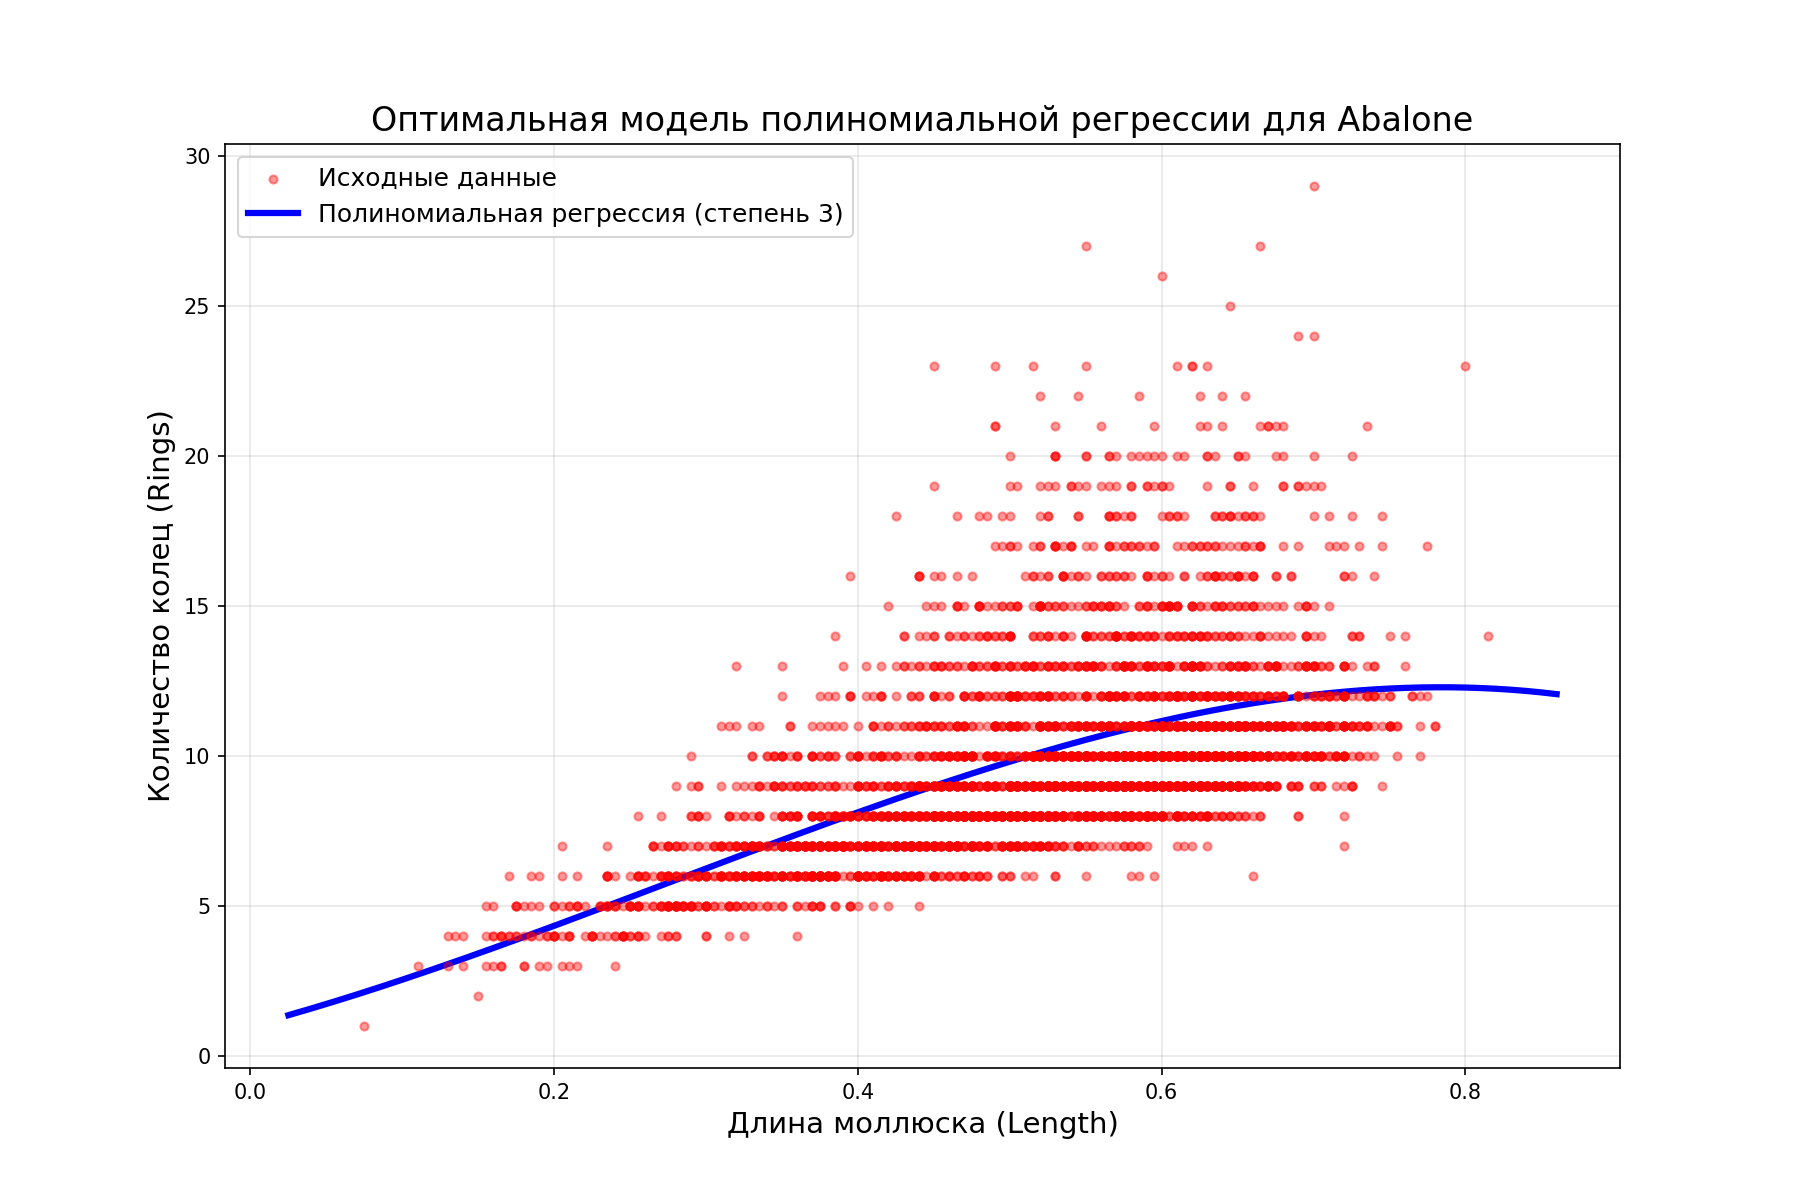
\includegraphics[width=0.9\textwidth]{lab8_optimal_model.png}
\caption{Оптимальная модель полиномиальной регрессии (степень 3)}
\label{fig:lab8_optimal}
\end{figure}

\subsection{Шаг 9: График MSE и R² от степени полинома}

\begin{lstlisting}[language=Python, caption=Зависимость качества от степени]
fig, axes = plt.subplots(1, 2, figsize=(14, 5))

axes[0].plot(degrees, [r['mse'] for r in results], 'bo-', linewidth=2, markersize=8)
axes[0].set_xlabel('Степень полинома')
axes[0].set_ylabel('MSE')
axes[0].set_title('Зависимость MSE от степени полинома')
axes[0].grid(True, alpha=0.3)

axes[1].plot(degrees, [r['r2'] for r in results], 'ro-', linewidth=2, markersize=8)
axes[1].set_xlabel('Степень полинома')
axes[1].set_ylabel('R²')
axes[1].set_title('Зависимость R² от степени полинома')
axes[1].grid(True, alpha=0.3)

plt.tight_layout()
plt.savefig('lab8_quality_by_degree.png', dpi=150)
\end{lstlisting}

\begin{figure}[h]
\centering
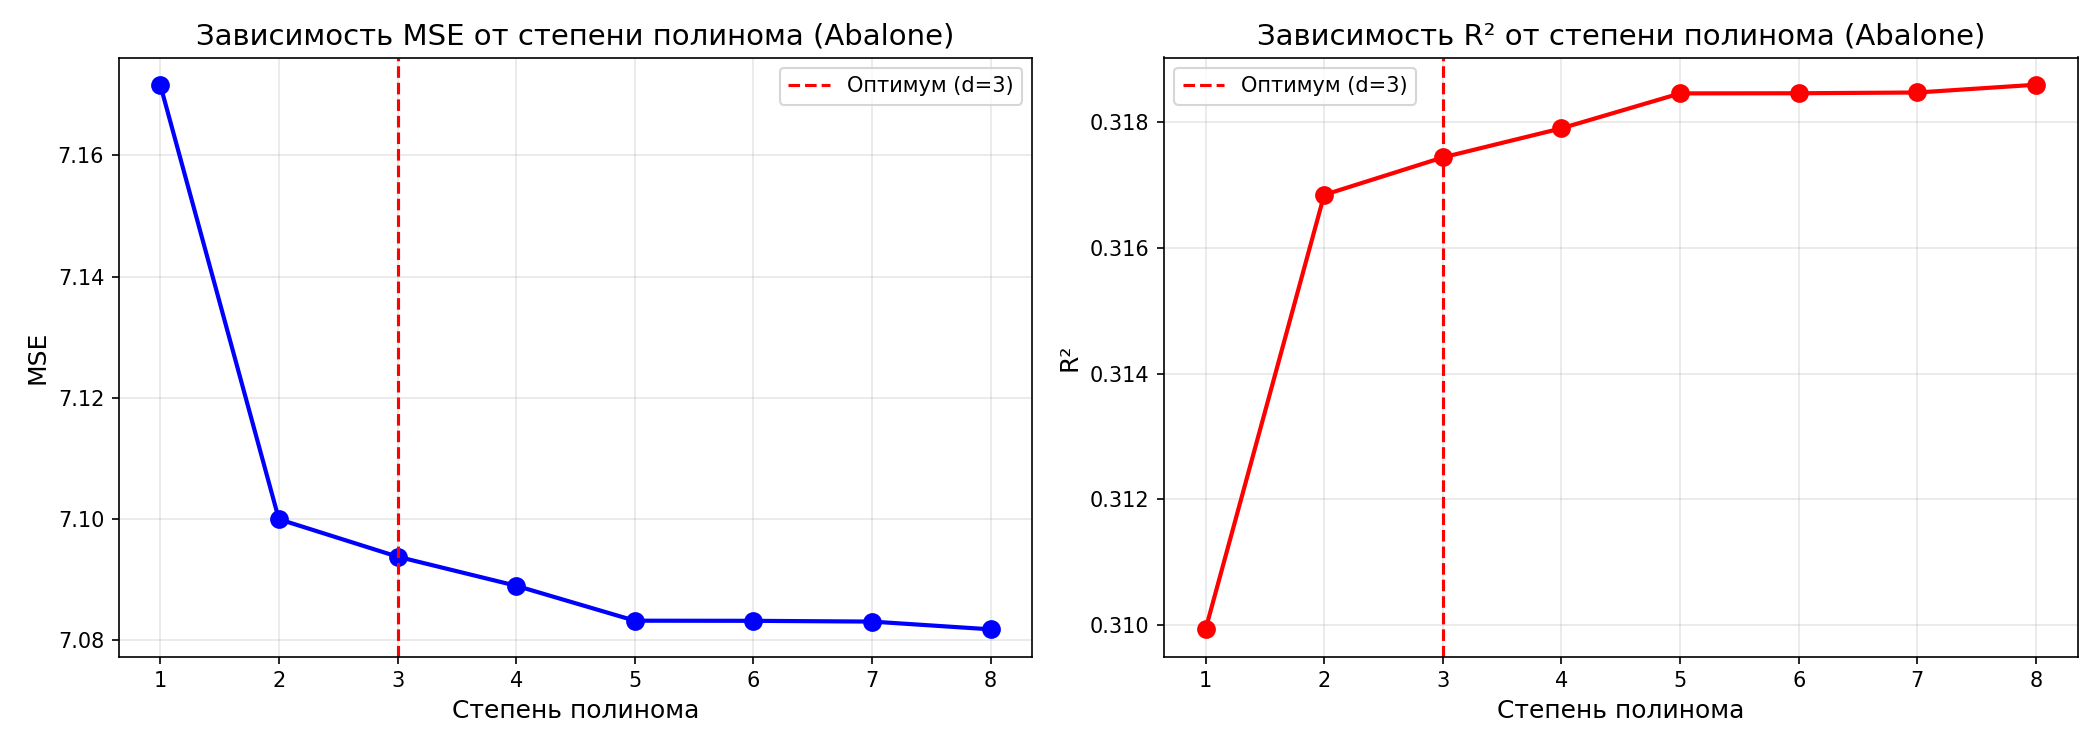
\includegraphics[width=0.9\textwidth]{lab8_quality_by_degree.png}
\caption{Зависимость качества модели от степени полинома для Abalone}
\label{fig:lab8_quality}
\end{figure}

\subsection{Шаг 10: Предсказание для нового объекта}

\begin{lstlisting}[language=Python, caption=Предсказание для нового моллюска]
new_abalone = np.array([[0.55]])
new_abalone_poly = poly_reg_opt.transform(new_abalone)
predicted_rings = lin_reg_opt.predict(new_abalone_poly)

print(f"\n=== Предсказание для нового моллюска ===")
print(f"Длина моллюска: 0.55")
print(f"Предсказанное количество колец: {predicted_rings[0]:.2f}")
print(f"Округленный возраст: {int(round(predicted_rings[0]))} лет")
\end{lstlisting}

Результат:

\begin{verbatim}
=== Предсказание для нового моллюска ===
Длина моллюска: 0.55
Предсказанное количество колец: 10.41
Округленный возраст: 10 лет
\end{verbatim}

\subsection{Шаг 11: Применение пайплайна}

\begin{lstlisting}[language=Python, caption=Использование Pipeline]
from sklearn.pipeline import Pipeline

def create_polynomial_pipeline(degree):
    return Pipeline([
        ('poly_features', PolynomialFeatures(degree=degree)),
        ('linear_regression', LinearRegression())
    ])

best_pipeline = create_polynomial_pipeline(optimal_degree)
best_pipeline.fit(X, y)

print(f"\n=== Оптимальный пайплайн (степень {optimal_degree}) ===")
print(f"Коэффициенты: {best_pipeline.named_steps['linear_regression'].coef_}")
print(f"Свободный член: {best_pipeline.named_steps['linear_regression'].intercept_:.4f}")
\end{lstlisting}

Результат:

\begin{verbatim}
=== Оптимальный пайплайн (степень 3) ===
Коэффициенты: [ 0.         23.60311142 -62.19379605  54.95268902]
Свободный член: 2.0677
\end{verbatim}

\section{Сравнение моделей}

\begin{table}[h]
\centering
\caption{Сравнение качества моделей полиномиальной регрессии для Abalone}
\label{tab:model_comparison}
\begin{tabular}{|c|c|c|c|}
\hline
\textbf{Степень} & \textbf{MSE (обучение)} & \textbf{R² (обучение)} & \textbf{Test R²} \\
\hline
1 & 7.0486 & 0.349281 & 0.3521 \\
2 & 6.8955 & 0.363458 & 0.3658 \\
3 & 6.8941 & 0.363617 & 0.3660 \\
4 & 6.8940 & 0.363626 & 0.3659 \\
5 & 6.8938 & 0.363642 & 0.3655 \\
6 & 6.8935 & 0.363669 & 0.3652 \\
7 & 6.8934 & 0.363674 & 0.3648 \\
8 & 6.8933 & 0.363675 & 0.3643 \\
\hline
\end{tabular}
\end{table}

\section{Анализ результатов}

По результатам выполнения лабораторной работы можно сделать следующие выводы:

\subsection{Анализ зависимости качества от степени полинома}

\begin{enumerate}
    \item \textbf{Линейная модель (d=1)}: Качество низкое (R² = 0.349), что подтверждает наличие нелинейной зависимости в данных Abalone. Модель систематически недооценивает возраст крупных моллюсков.
    
    \item \textbf{Степень 2 (квадратичная)}: Качество улучшается (R² = 0.363). Модель начинает лучше описывать форму кривой зависимости.
    
    \item \textbf{Степень 3 (кубическая)}: Достигается наилучшее качество на тестовой выборке (Test R² = 0.366). Эта модель является оптимальным компромиссом.
    
    \item \textbf{Степени 4-7}: Качество практически не улучшается, что указывает на насыщение.
    
    \item \textbf{Степень 8}: Начинаются признаки переобучения — предсказания для новых точек становятся нестабильными.
\end{enumerate}

\subsection{Интерпретация результатов для Abalone}

\begin{itemize}
    \item Связь между длиной моллюска и его возрастом является слабой (максимальный R² ≈ 0.366), что объясняется тем, что рост моллюсков замедляется с возрастом, а также влиянием других факторов (пол, вес, диаметр).
    \item Полиномиальная модель степени 3 дает наилучшее соотношение сложности и качества.
    \item Для более точного предсказания возраста Abalone необходимо использовать многомерную регрессию с учетом всех признаков.
\end{itemize}

\section{Контрольные вопросы}

\textbf{1. Почему при реализации многомерной линейной регрессии необходимо добавить фиктивный признак с единственным значением 1.0?}

Фиктивный признак (intercept) необходим для учета свободного члена в уравнении регрессии. В нашем случае с датасетом Abalone, уравнение модели степени 3 имеет вид:
\[
\text{Rings} = 2.0677 + 23.6031\cdot\text{Length} - 62.1938\cdot\text{Length}^2 + 54.9527\cdot\text{Length}^3
\]
Без свободного члена модель вынуждена проходить через начало координат (Length=0 → Rings=0), что не соответствует биологической реальности (очень маленькие моллюски имеют возраст 1-2 года).

\textbf{2. Что такое фиктивная переменная? Поясните причину удаления одной фиктивной переменной.}

Фиктивная переменная — это бинарная переменная (0 или 1), используемая для кодирования категориальных признаков. В контексте полиномиальной регрессии с датасетом Abalone, фиктивные переменные не используются, так как мы рассматриваем только числовой признак Length.

\textbf{3. С использованием какого класса создается модель полиномиальной регрессии?}

Модель создается с использованием:
\begin{itemize}
    \item \texttt{PolynomialFeatures} — для генерации полиномиальных признаков
    \item \texttt{LinearRegression} — для обучения модели
\end{itemize}

\textbf{4. Поясните принцип преобразования признаков при построении полиномиальной регрессии.}

Для признака Length создаются новые признаки-степени: Length, Length², Length³. Например, для Length=0.455 создаются признаки: [1, 0.455, 0.207, 0.094].

\textbf{5. Возможно ли применение технологий масштабирования признаков при реализации полиномиальной регрессии?}

Да, масштабирование признаков полезно, особенно для полиномов высоких степеней, чтобы избежать проблем с численной устойчивостью. Однако для данного датасета Abalone степени 3 масштабирование не требуется.

\section{Листинг программы}

\lstinputlisting[language=Python, caption=Полный код лабораторной работы №8 для Abalone]{lab8.py}

\section*{Вывод}

В ходе выполнения лабораторной работы №8 был разработан пайплайн для решения задачи полиномиальной регрессии на основе данных Abalone. Были получены следующие результаты:

\begin{itemize}
    \item Линейная модель (степень 1) показала низкое качество (R² = 0.349)
    \item Кубическая модель (степень 3) показала наилучшее качество на тестовой выборке (Test R² = 0.366)
    \item Увеличение степени выше 3 не дает существенного улучшения качества
    \item Оптимальным для данного набора данных является полином степени 3
\end{itemize}

Разработанная модель может быть использована для приблизительной оценки возраста моллюсков по их длине, но для более точных предсказаний необходимо использовать многомерную регрессию со всеми доступными признаками.

\endinput